\documentclass{article}
\usepackage{graphicx} % Required for inserting images
\usepackage{amsmath}
\usepackage{amsfonts}
\usepackage{amssymb}

\title{Transformation \& Simulation Methods}
\author{Max Lang}
\date{January 2024}

\begin{document}

\maketitle
\section{Box-Muller algorithm}
\subsection{Intuitive Explanation}

The Box-Muller algorithm is a method for generating normally distributed random numbers from uniformly distributed random numbers. It's a fascinating transformation that bridges the gap between these two types of distributions. Here's an intuitive explanation:

\begin{enumerate}
    \item Start with two independent uniformly distributed random numbers \( U_1 \) and \( U_2 \).
    \item Transform these numbers into polar coordinates. This involves thinking of \( U_1 \) and \( U_2 \) as representing a point in a circle.
    \item Apply specific mathematical functions involving exponentials and trigonometric functions to these polar coordinates.
    \item The transformed numbers now follow a normal distribution, characterized by a higher density of values near the mean.
\end{enumerate}

\subsection{Mathematical Explanation}

Mathematically, the Box-Muller algorithm is expressed through the following steps:

\begin{enumerate}
    \item Start with two independent uniformly distributed random variables \( U_1, U_2 \sim \text{Uniform}(0, 1) \).
    \item Convert to polar coordinates:
    \begin{itemize}
        \item Calculate \( R^2 = -2 \ln(U_1) \)
        \item Calculate \( \Theta = 2\pi U_2 \)
    \end{itemize}
    \item Transform to normally distributed variables:
    \begin{itemize}
        \item Calculate \( Z_0 = \sqrt{-2 \ln(U_1)} \cos(2\pi U_2) \)
        \item Calculate \( Z_1 = \sqrt{-2 \ln(U_1)} \sin(2\pi U_2) \)
    \end{itemize}
\end{enumerate}

These steps convert the uniform distribution of \( U_1 \) and \( U_2 \) into a normal distribution for \( Z_0 \) and \( Z_1 \).
\begin{figure}
    \centering
    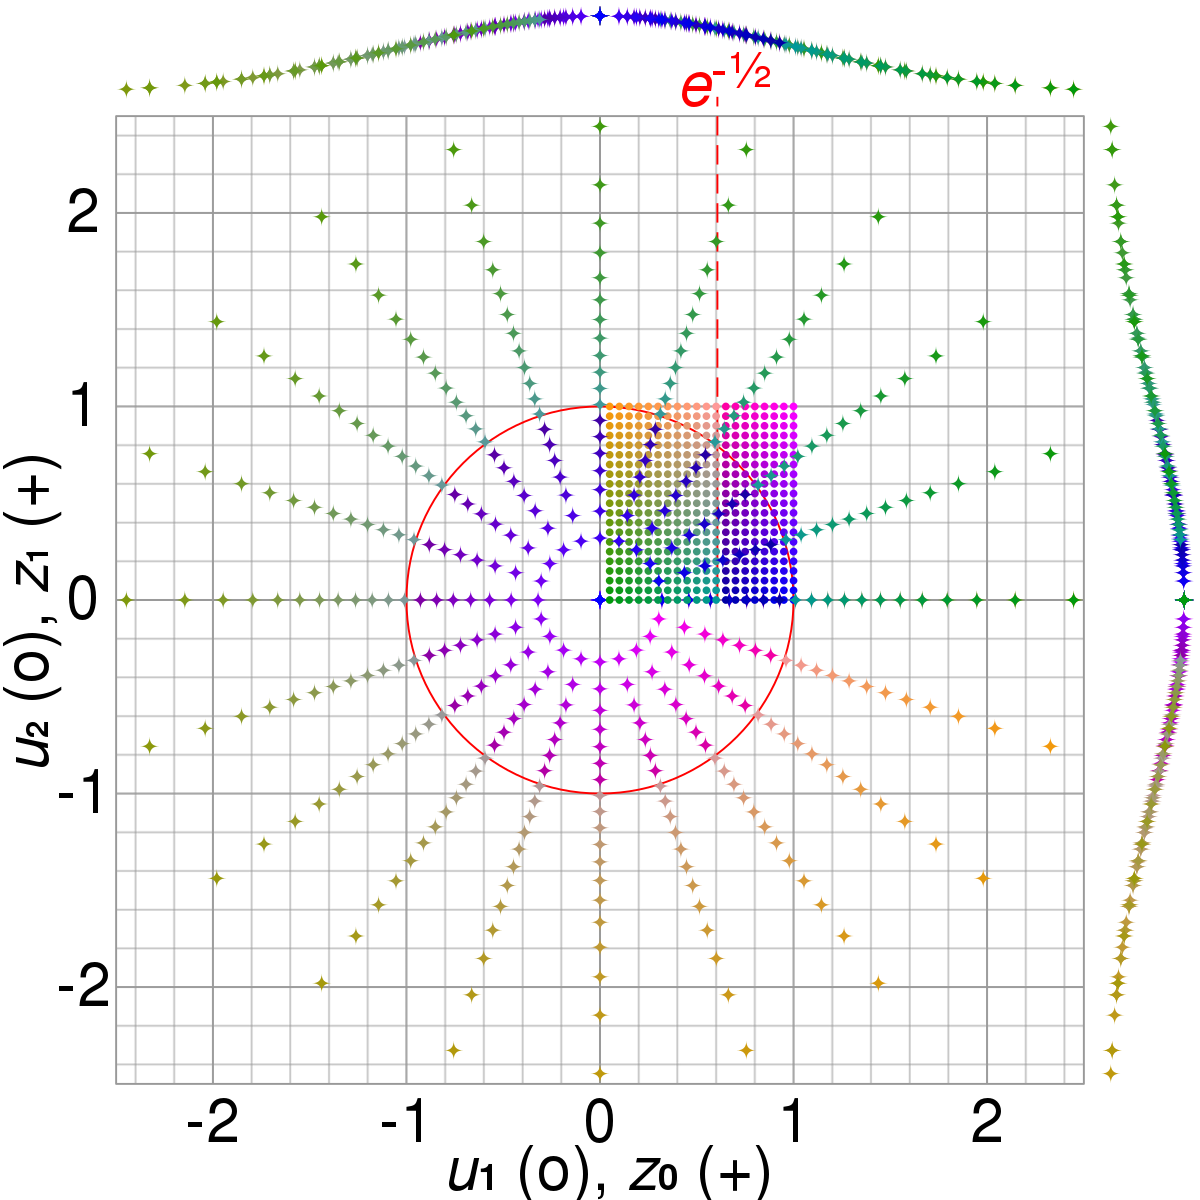
\includegraphics[width=0.5\linewidth]{figures/1200px-Box-Muller_transform_visualisation.svg.png}
    
    
\end{figure}
\begin{figure}
    \centering
    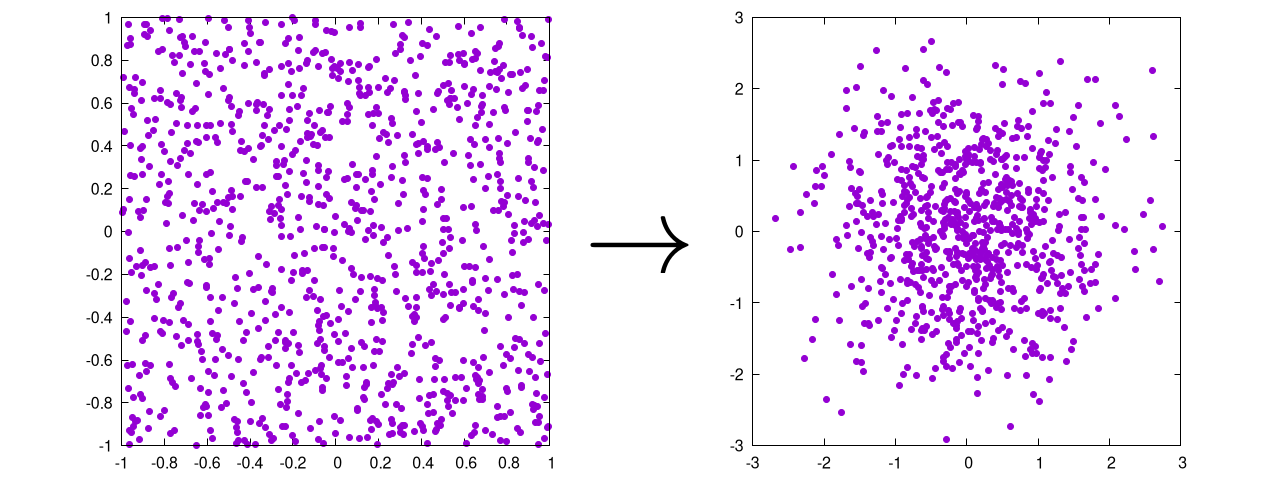
\includegraphics[width=0.75\linewidth]{ox-hilary/simulation-methods/figures/polar_rand_transform.png}
\end{figure}
\begin{figure}
    \centering
    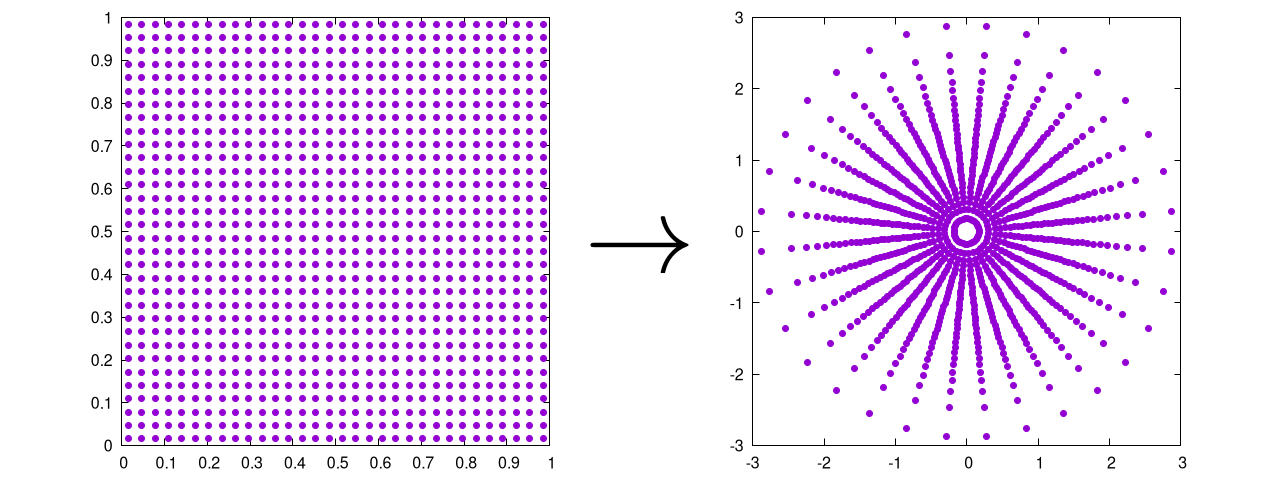
\includegraphics[width=0.75\linewidth]{ox-hilary/simulation-methods/figures/cartesian_grid_transform.png}
\end{figure}
\begin{figure}
    \centering
    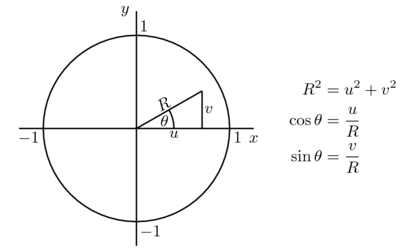
\includegraphics[width=0.75\linewidth]{ox-hilary/simulation-methods/figures/400px-BoxMullerTransformUsingPolarCoordinates.png}
\end{figure}

\section{Sampling via compostion}
\subsection{Intuitive Explanation}
Sampling via composition is a method used to sample from a complex distribution that is made up of several simpler distributions. The idea is similar to building a model out of Lego blocks: instead of trying to carve the entire model out of a single block of plastic (which would be difficult), you assemble it from individual Lego blocks that are easy to handle.

Here's an everyday scenario to understand this better: suppose you're making a sandwich with various ingredients. Each ingredient represents a simpler distribution. You can choose each ingredient (sample from each simpler distribution) independently and then combine them to make your sandwich (the complex distribution). This is essentially what composition is about: combining simpler parts to form a whole.
\begin{enumerate}
    \item Decomposition: Assume you have a joint probability distribution $\pi(x, y)$ that you want to sample from. This joint distribution can often be decomposed into its marginal distribution $\pi(x)$ and conditional distribution $\pi(y \mid x)$.
    \item Sample from Marginal Distribution: First, you sample $x$ from its marginal distribution $\pi(x)$.
    \item Sample from Conditional Distribution: Then, for each sampled $x$, you sample $y$ from the conditional distribution $\pi(y \mid x)$.
\end{enumerate}

By doing this, you obtain a sample $(x, y)$ from the joint distribution $\pi(x, y)$. Mathematically, if $X$ and $Y$ are two random variables with joint distribution $\pi(x, y)$, you can express it as:
$$
\pi(x, y)=\pi(x) \cdot \pi(y \mid x)
$$
where $\pi(x)$ is the probability of $x$ independently, and $\pi(y \mid x)$ is the probability of $y$ given that $x$ has occurred.

This method is particularly useful when it's easier to sample from the marginal and conditional distributions than from the joint distribution directly. It's a divide-and-conquer strategy applied to the problem of sampling from probability distributions.

\section{Rejection sampling}
\subsection{Intuitive Explanation}
The rejection sampling algorithm, also known as acceptance-rejection method, is a basic technique used to generate observations from a distribution. It is particularly useful when direct sampling is difficult. The intuition behind rejection sampling can be understood through a simple analogy:

Imagine you have a dartboard, which represents the probability distribution you want to sample from. However, this dartboard has a complicated shape and is not easy to aim at directly. So instead, you use a larger, rectangular dartboard that completely covers the original one. This rectangle represents a simpler distribution from which you can easily draw samples, often called the proposal distribution.

Now, you throw darts randomly at the larger rectangle. Whenever a dart lands within the bounds of the original complicated dartboard, you accept the throw as a sample from your desired distribution. If the dart lands outside of it but still within the rectangle, you reject it and throw again.

This process ensures that the proportion of accepted darts will represent the complex probability distribution you're interested in, even though you're sampling from a simpler distribution.

\begin{figure}
    \centering
    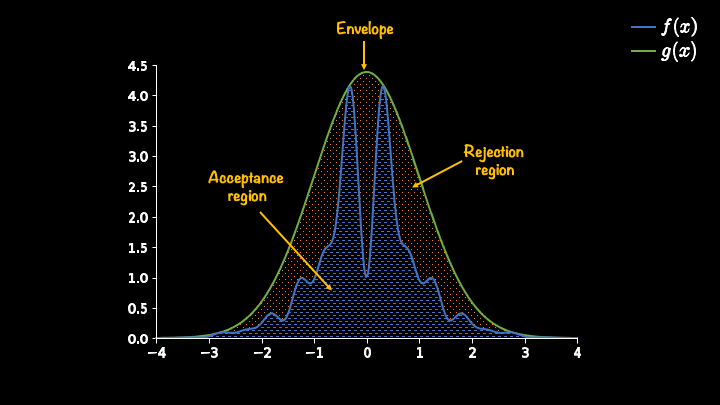
\includegraphics[width=1\linewidth]{ox-hilary/simulation-methods/figures/1_Y8v8ASUKQxeWDHSDTJb7aA.png}
\end{figure}

\subsection{Mathematical Explanation}
Mathematically, rejection sampling follows these steps:
\begin{enumerate}
    \item Choose a Proposal Distribution: Select a proposal distribution, $q(x)$, from which you can easily sample, and a constant $c$ such that $c \cdot q(x)$ is always greater than or equal to your target distribution $p(x)$ for all $x$.
    \item Sample from the Proposal Distribution: Generate a sample, $x$, from $q(x)$.
    \item  Calculate Acceptance Probability: Compute the acceptance probability as $\frac{p(x)}{c \cdot q(x)}$.
    \item Decide to Accept or Reject: Generate a uniform random number, $u$, between 0 and 1 . If $u$ is less than or equal to the acceptance probability, accept $x$ as a sample from $p(x)$; otherwise, reject $x$.
    \item  Repeat: Continue this process until you have enough accepted samples.
\end{enumerate}

This algorithm leverages the fact that scaling up the proposal distribution and then selectively accepting samples can simulate the more complicated target distribution. The constant $c$ ensures that the scaled-up proposal distribution always encompasses the target distribution, making sure that every part of the target distribution has a chance to be sampled. The acceptance probability corrects for the areas where the proposal distribution is too large, leading to an accurate representation of the target distribution.

\subsection{Algorithm}

Given two densities $\pi, q$ on $\mathrm{X}$ with $\pi(x) \leq M q(x)$ for all $x \in \mathbb{X}$ and some $M<\infty$, we can generate a sample from $\pi$ as follows:
\newline
1. Draw $X \sim q$.
\newline
2. Accept $X=x$ as a sample from $\pi$ with probability
$$
\alpha=\frac{\pi(x)}{M \cdot q(x)},
$$
otherwise go back to step 1 .
\newline
Note that to implement rejection sampling, we need to implement a mechanism to either "do this" or "do that" according to some probability $\alpha \in[0,1]$. The standard way to implement this goes as follows.\newline
\newline
1. Draw $U \sim \mathcal{U}_{[0,1]}$. \newline
2. If $U \leq \alpha$ then "do this", otherwise "do that".
\newline
Indeed $\mathbb{P}(U \leq \alpha)=\alpha$ when $U \sim \mathcal{U}_{[0,1]}$, so that the above scheme will "do this" with probability $\alpha$.



\section{Importance Sampling}
\subsection{Intuitive Explanation}
Importance sampling is a technique used to estimate properties of a particular distribution, while only having samples from a different distribution. This method is especially useful when it is difficult to sample directly from the distribution of interest. The core idea behind importance sampling can be illustrated with a straightforward analogy:

Imagine you're trying to understand the behavior of a rare bird species in a vast forest, but these birds are so scarce that finding them by random search would be inefficient. Instead, you decide to focus on specific parts of the forest where birds are known to visit more frequently, based on previous observations or expert knowledge. These parts represent the proposal distribution from which you can more easily collect samples.

Once you have your observations, you don't just count the birds seen; you also weigh each observation by how representative it is of the entire forest. This weighting corrects for the bias introduced by focusing on the specific parts of the forest, allowing you to estimate the total bird population or other characteristics accurately.

\subsection{Mathematical Explanation}
Mathematically, importance sampling involves the following steps:
\begin{enumerate}
    \item Choose a Proposal Distribution: Select a proposal distribution, $q(x)$, from which you can easily sample. Ideally, $q(x)$ should be similar to your target distribution $p(x)$ but easier to sample from.
    \item Compute Weights: For each sample $x$ drawn from $q(x)$, compute a weight $w(x) = \frac{p(x)}{q(x)}$. This weight measures how much more (or less) likely the sample is under the target distribution compared to the proposal distribution.
    \item Estimate Target Properties: Use the weighted samples to estimate properties of the target distribution, such as its mean or variance. For example, the weighted average of the samples can estimate the expected value under the target distribution.
\end{enumerate}

This process leverages the proposal distribution to efficiently explore the sample space, with the weights correcting for the difference between the proposal and target distributions. This correction allows for accurate estimation of the target distribution’s properties without directly sampling from it.

\subsection{Algorithm}

To estimate the expected value of a function $f(x)$ under the target distribution $\pi(x)$ using samples from a proposal distribution $q(x)$, we follow these steps:
\newline
1. Draw $n$ independent samples $X_1, X_2, \ldots, X_n$ from $q(x)$.
\newline
2. Compute weights for each sample: $w_i = \frac{\pi(X_i)}{q(X_i)}$ for $i = 1, 2, \ldots, n$.
\newline
3. Estimate the expected value as:
$$
\hat{E}[f(X)] = \frac{\sum_{i=1}^n w_i f(X_i)}{\sum_{i=1}^n w_i}.
$$


\subsection{Standard Importance Sampling}

Let \( q \) and \( \pi \) be two probability density functions on \( \mathcal{X} \) such that \( \pi(x) > 0 \) implies \( q(x) > 0 \). Then, for any set \( A \) such that \( \pi(A) > 0 \)

\[
\pi(A) = \int_A \frac{\pi(x)}{q(x)}q(x)dx = \int_A w(x)q(x)dx
\]

where \( w: \mathcal{X} \rightarrow \mathbb{R}^+ \) is the so-called importance weight function: \( w: x \mapsto \frac{\pi(x)}{q(x)} \). This identity can be obviously generalized to the expectation of any function. Assume \( \pi(x)\phi(x) > 0 \) implies \( q(x) > 0 \), then

\[
I = \mathbb{E}_{\pi}[\phi(X)] = \int_{\mathcal{X}} \phi(x) \pi(x) dx = \int_{\mathcal{X}} \phi(x) w(x) q(x) dx = \mathbb{E}_q[\phi(X)w(X)].
\]

Now let \( X_1, \ldots, X_n \) be a sample of independent random variables distributed according to \( q \), then the estimator

\[
\hat{I}_{\text{IS}} = \frac{1}{n} \sum_{i=1}^{n} \phi(X_i)w(X_i)
\]

is consistent through the strong law of large numbers if \( \mathbb{E}_q[|\phi(X)|w(X)] < \infty \). We also obtain the following results.

\textbf{Bias and Variance of Standard Importance Sampling}
\begin{itemize}
    \item[(a)] \( \mathbb{E}_q \left[ \hat{I}_{\text{IS}} \right] = I \),
    \item[(b)] \( \text{Var}_q \left( \frac{\hat{I}_{\text{IS}}}{n} \right) = \frac{1}{n} \text{Var}_q(\phi(X)w(X)) \) and if \( \sigma^2_{\text{IS}}(\phi) = \text{Var}_q(\phi(X)w(X)) < \infty \),
    \item[(c)] \( \sqrt{n} \left( \frac{\hat{I}_{\text{IS}}}{n} - I \right) \rightarrow \mathcal{N}(0, \sigma^2_{\text{IS}}(\phi)) \).
\end{itemize}

\subsection{Normalised Importance Sampling}

\subsubsection{Challenge with Standard Importance Sampling}

The challenge with standard importance sampling arises when we need to know the exact form of \( \pi(x) \), the target distribution. In many practical applications, especially in Bayesian inference, we only know \( \pi(x) \) up to a constant factor, because calculating the normalising constant \( Z_{\pi} \) (which makes the integral of \( \pi(x) \) over its support equal to 1) can be difficult or computationally infeasible.

\subsubsection{Normalised Importance Sampling}

Normalised importance sampling addresses this challenge by using an unnormalised version of the target distribution \( \tilde{\pi}(x) \) and the proposal distribution \( \tilde{q}(x) \). Here's what normalising means in this context:

\subsubsection{Unnormalised Distributions}

Both \( \tilde{\pi}(x) \) and \( \tilde{q}(x) \) are the forms of the distributions without being scaled by their respective normalising constants. That is, they can be used to calculate probabilities, ratios of probabilities, or expectations, but their integrals over all possible values of \( x \) do not necessarily sum or integrate to 1.

\subsubsection{Normalising Constants}

\( Z_{\pi} \) and \( Z_q \) are the normalising constants for \( \tilde{\pi}(x) \) and \( \tilde{q}(x) \), respectively. These constants are what you would multiply the unnormalised functions by in order to make them proper probability distributions (i.e., so that they integrate to 1 over the space of \( x \)). They are often difficult to compute, which is why methods that avoid needing them explicitly, like normalised importance sampling, are useful.

\subsubsection{How Normalised Importance Sampling Works}

In normalised importance sampling, we work with unnormalised weights derived from the unnormalised distributions. The weight for a sample \( x \) drawn from \( q(x) \) is given by the ratio of the unnormalised target and proposal densities at \( x \):

\[ w(x) = \frac{\tilde{\pi}(x)}{\tilde{q}(x)} \]

Since both \( \tilde{\pi}(x) \) and \( \tilde{q}(x) \) are unnormalised, the weights \( w(x) \) do not depend on the unknown normalising constants \( Z_{\pi} \) and \( Z_q \). This allows for the estimation of expectations under \( \pi(x) \) without knowing these constants.

\subsubsection{Final Estimation}

In practice, standard importance sampling has limited applications as it requires exact evaluations of \( \pi(x) \), contrarily to rejection sampling where \( \pi(x) \) and \( q(x) \) only have to be evaluated up to some normalising constants. However there is an alternative version of importance sampling known as normalised importance sampling which bypasses this problem. Assume that whenever \( \pi(x) > 0 \) implies \( q(x) > 0 \), and that we can write \( \pi(x) = \tilde{\pi}(x)/Z_{\pi} \) and \( q(x) = \tilde{q}(x)/Z_q \), for some normalising constants \( Z_{\pi} \) and \( Z_q \). We introduce the unnormalised weight function

\[
\tilde{w}: x \mapsto \frac{\tilde{\pi}(x)}{\tilde{q}(x)} = w(x)\frac{Z_{\pi}}{Z_q}.
\]

Then, we can write

\[
I = \mathbb{E}_{\pi}[\phi(X)] = \int_{\mathcal{X}} \phi(x) \pi(x) dx = \int_{\mathcal{X}} \phi(x) \tilde{w}(x)q(x) dx = \int_{\mathcal{X}} \phi(x) w(x) \tilde{q}(x) dx = \mathbb{E}_q[\phi(X)\tilde{w}(X)].
\]

where the importance weight function only involves the \textbf{unnormalised probability density functions \( \tilde{\pi} \) and \( \tilde{q} \).}

Now, let \( X_1, \ldots, X_n \) be a sample of independent random variables distributed according to \( q \). The estimator

\[
\hat{I}_{\text{NIS}} = \frac{\sum_{i=1}^{n} \phi(X_i)\tilde{w}(X_i)}{\sum_{i=1}^{n} \tilde{w}(X_i)}
\]

is consistent through the strong law of large numbers as long as \( \mathbb{E}_q[|\phi(X)|\tilde{w}(X)] < \infty \). The normalised importance sampling estimator \( \hat{I}_{\text{NIS}} \) is a ratio of two estimators, therefore we do not have simple expressions for its finite bias and variance. We can still obtain their asymptotic expression (i.e. as \( n \rightarrow \infty \)) using the delta method.


\begin{figure}
    \centering
    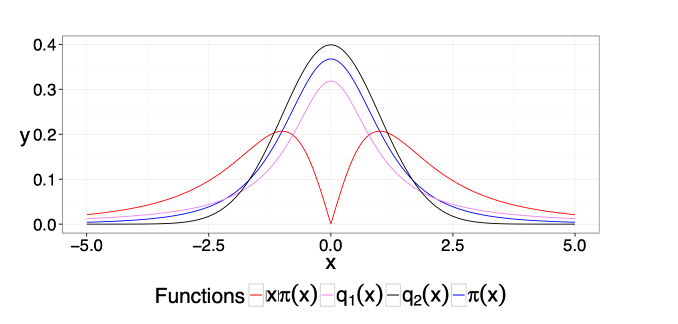
\includegraphics[width=0.75\linewidth]{ox-hilary//simulation-methods//figures/NIS_dist.png}
    \caption{Different importance proposal distributions to estimate the area under the red curve.  
}
    \label{fig:nis_dist}
\end{figure}
\begin{figure}
    \centering
    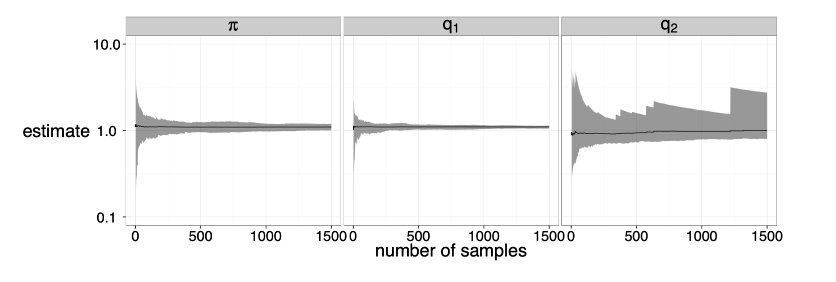
\includegraphics[width=0.75\linewidth]{ox-hilary//simulation-methods//figures/NIS_burn_in.png}
    \caption{Estimates of $I$ obtained after 1 to 1500 samples, using proposals $\pi$ (left), $q_1$ (middle) or $q_2$ (right). The grey shaded areas correpond to the range of 100 independent replications, and the black line represents the mean.}
    \label{fig:nis_burn_in}
\end{figure}
\begin{figure}
    \centering
    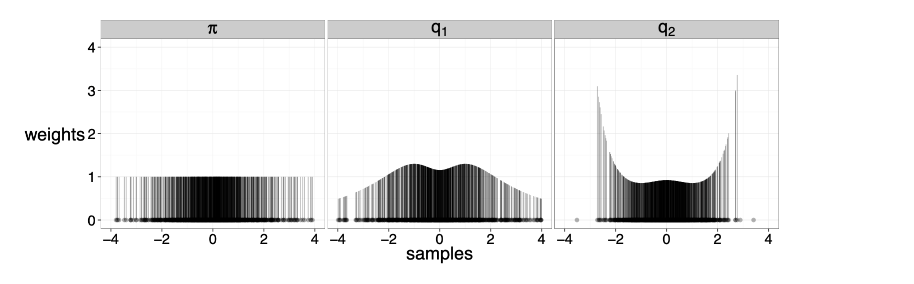
\includegraphics[width=0.75\linewidth]{ox-hilary//simulation-methods//figures/NIS_weights.png}
    \caption{Sample weights obtained for 1000 realisations of $X_i$, using proposals $\pi$ (left), $q_1$ (middle) or $q_2$ (right).}
    \label{fig:nis_weights}
\end{figure}
\end{document}
